\documentclass[a4paper,11pt]{article}

\usepackage{graphicx}
\usepackage{natbib}
\usepackage[utf8]{inputenc}
\usepackage{tabularx}
\usepackage{hyperref}
\usepackage{color}
\usepackage{float}
\usepackage[usenames,dvipsnames,svgnames,table]{xcolor}
% \usepackage{mathptmx} % Times New Roman

\setlength{\topmargin}{-0.4mm} % (1in=25.4mm)-0.4mm=25mm
\setlength{\textheight}{243.119mm} % 297mm-40mm-10mm-(11pt=3.881mm)=
\setlength{\oddsidemargin}{-0.4mm} % (1in=25.4mm)-0.4mm=25mm
\setlength{\textwidth}{160mm} % 210mm-50mm=160mm
\setlength{\headheight}{0mm}
\setlength{\headsep}{0mm}
\setlength{\footskip}{15mm}

\providecommand*{\note}[1]{\small \textcolor{RoyalBlue}{\begin{minipage}{\textwidth}{#1}\end{minipage}}}

% --------------------------------------------------------------

\providecommand*{\ShortTitle}{WaveMeIn}
\providecommand*{\FullTitle}{WaveMeIn: Authentication via Brain Waves}

% --------------------------------------------------------------

\title{\textbf{\sffamily\Huge \ShortTitle}\\ 
{\textbf{\sffamily\Large \FullTitle}}
\vspace{1cm}}

\author{
{\em 188.407: Management von Software Projekten} \vspace{1cm} \\
Group: 10\bigskip \\
Belk Stefan \\ {\small 0750926, 937, \href{mailto:belk.stefan@gmail.com}{belk.stefan@gmail.com}}\\
Petz Thomas \\ {\small 0601280, 937, \href{mailto:e0601280@student.tuwien.ac.at}{e0601280@student.tuwien.ac.at}}\\
Causevic Alma \\ {\small 0847805, 534, \href{mailto:alma.causevic@hotmail.com}{alma.causevic@hotmail.com}}\\ 
Causevic Amra  \\ {\small 0649241, 534, \href{mailto:amra.causevic@hotmail.com}{amra.causevic@hotmail.com}}\\ 
Seebacher David \\ {\small 0327243, 534, \href{mailto:david.seebacher@student.tuwien.ac.at}{david.seebacher@student.tuwien.ac.at}}\\
\vspace{4cm}
}

\begin{document}

\begin{titlepage}
\maketitle

\end{titlepage}

% --------------------------------------------------------------

\thispagestyle{empty}
\tableofcontents
\pagebreak

\setcounter{page}{1}


% --------------------------------------------------------------

\note{
\textbf{Formal constraints}
\begin{itemize}
\item	  Font: Times New Roman oder Computer Modern (\LaTeX default)
\item    Fontsize: 11pt
\item     Single line spacing
\item     Margins: 2.5cm side and top/bottom
\item     \fbox{Language: ENGLISH}
\item    The proposal template should be filled incrementally. I.e., at the end there should be a full project proposal in a single PDF file.
\end{itemize}
\textbf{Available templates}
\begin{itemize}
\item     Proposal (mswp-proposal.tex)
\item     Costs (costs.xls, costs.ods)
\end{itemize}
\textbf{Supplemental material}
\begin{itemize}
\item     FWF salary scheme (\href{http://www.fwf.ac.at/de/projects/personalkostensaetze.html}{http://www.fwf.ac.at/de/projects/personalkostensaetze.html})
\item     Travel cost regulation (\href{http://www.fwf.ac.at/de/faq/reisegebuehrenvorschrift.html}{http://www.fwf.ac.at/de/faq/reisegebuehrenvorschrift.html})
\item     Ethical issues form (ethical-issues.rtf)
\end{itemize}
}
\pagebreak

% --------------------------------------------------------------
\section{Synopsis}
\label{sect:synopsis}
\subsection{Project Idea}
WaveMeIn is a research project to create a new type of secure login mechanism. It consists of a small device worn by the user at the ear which authenticates the user based on brain waves.

\subsection{Why do we need it?}
At the time of this proposal the most used ways for authentication are manually typed passwords or biometric authentication methods. However all of the previous methods have some security problems or are simply not user-friendly. Typed passwords are easy to spy out simply by looking at the keyboard of the user or the traces of the fingers on touch displays. In the case of biometric authentication, there are for example face recognition, iris or fingerprint scans. Face recognition software can easily be tricked by face masks or photographs and moreover depends on good light conditions, the quality of the images of the web camera and other factors. Fingerprint and iris scans are the most secure options of the authentication methods mentioned before. However they also have many disadvantages. Iris scans are not practical since the hardware required cannot easily be integrated into small devices and it is not user-friendly to require the user to place his eye very close to the scanner every time he/she wants to unlock a device. Fingerprint sensors are known to fail to recognize the fingerprint correctly quite often and it is also a not very user-friendly authentication method for handicapped people that may not reach the sensor or may not have any fingers at all. 

\subsection{How does it work?}
Brain waves are a secure and user-friendly alternative authentication method. The idea is to create a small device, called Wavy, that can be worn at the ear of the user in the same style as bluetooth headsets are already worn for communication today. The Wavy measures the brain waves near the ear in case a login is required by a client device that is connected via bluetooth. It listens for a brain wave pattern that was previously trained by the user as a password. If the correct pattern was detected by the Wavy it transmits a OK signal back to the client device. 

\subsection{Why should somebody care?}
Nowadays people are forced to type their passwords in public places which is a security risk and also not a very efficient way for authentication. Especially when typing in password on small devices such as mobile phones this authentication method is also very error prone due to the small keyboard interfaces. On the one side people are lazy and do not want to remember and enter long and complicated passwords, but on the other side they are also concerned about the security of their data and their privacy. So the users are in need of a more secure and easier way of authentication.

\subsection{Who are the beneficiaries of the results?}
Basically everybody can benefit from the WaveMeIn project since it is usable in the daily life. Especially for handicapped people it is a new and more easy to use option to log into their devices. Also it grants a higher level of security than existing authentication methods so it is also well suited for environments where higher security is needed, such as access authentication is modern research labs and government or military facilities.

For our product to succeed, we need to invest into research in the area of brain wave detection and analysis. This investment can improve our understanding of this topic. After a commercial success, we have to enhance our product. This means we have to invest further into brain wave research. On the other side, we can make our world more secure. It makes hacking of accounts and password fraud more complicated.

\subsection{Problem classification}
The task of detecting brain waves it tightly connected to the research areas of Neuroscience, Pattern Recognition and Machine Learning. In the field of Neuroscience it touches the areas of not invasive brain computer interfaces and neural oscillation. Since detecting and reliably identifying brain waves at the location near the ears is still technically immature the project can be seen as basic research in this area. The following research questions have to be answered before a prototype can be developed.
\begin{itemize}
	\item Detecting braves at the ears
	\item Recognize brain wave patters
	\item Distinguish correct patterns from random signals
	\item Distinguish brain waves from different users
\end{itemize}
On the other hand if we take the Wavy into account, which should be the resulting product, this project is also an applied research project. It further touches the fields of computer security and privacy.


% --------------------------------------------------------------
\section{Introduction and problem description}
\label{sect:intro}
WaveMeIn is a research project to show the potential of brain waves a new method of electronic authentication via a small wearable device. Its aim is to investigate the usage of rain waves to replace passwords or other authentication methods. Therefore the properties of brain waves regarding uniqueness and reliability have to be explored. The project shall demonstrate via a small prototype that the recognition is possible without large sensors on top of the users head. A requirement for such a method of authentication clearly exists as demonstrated by the following use cases:

\subsection{Current Situation}


\subsection{Use Case 1}{
Assume a user needs to log on to a device (e.g. a notebook) that contains sensitive information in public. Typing in the password is not an option as it can easily be monitored by another person. Fingerprints are also not a good alternative as they can easily be taken from any surface the user touched and be copied onto synthetic materials to deceive the fingerprint reader. Brain waves are (as of current knowledge) unique for each person even if two people are having exactly the same thought. If the intruder does not know the precise brain wave pattern of the user's pass phrase/thought it is impossible to duplicate.}

\subsection{Use Case 2}{
Assume an average user wants to unlock his/her smart phone in a crowded area such as the subway. Nowadays this is done by entering a pin or drawing a pattern on the screen. A person with the intention to steal a users phone just needs to observe its victim while entering the pass code or pattern. Afterwards it is easy to unlock the phone and steal the victims personal data or cause large costs while using it for phone calls and mobile data. Locking the phone via a brain wave authentication mechanism may not prevent the theft but the costs arising from the phone being used afterwards.}

\subsection{Current Authentication Methods}
In theory brain waves will be rank among the most secure authentication methods, probably being the most secure one if the research proves successful. The particular brain wave of a user required to unlock a device can not be easily be obtained other than strapping the user to a chair and forcing him/her to think his/her pass thought. Other authentication methods are password, drawing patterns, fingerprint, iris scan, voice recognition. Passwords and pattern drawing are the least secure ones as the user can be observed while typing or drawing without much effort. Fingerprint, iris scan, voice recognition may require more technical or social effort to obtain, but in the end all of them are features of a person that are always visible for the outside world and therefore copyable with more or less effort.

\subsection{Unresolved Problems and Opportunities}
The unknown factor of this research project is that no research has been done on measuring brain waves at other locations (e.g. the ears) of the body except directly at the users head. Additionally it is unknown if the brain waves of are person are distinctive enough to distinguish a pass thought of a user from other thoughts and if the brain waves of different users while thinking the same thought are distinctive enough.

At the time of writing this proposal there exists no device that is capable of the features mentioned above as well as being small enough to be worn as an accessory. Therefore this is an important area of research with practical future applications.

\subsection{Terms}
\begin{itemize}
	\item 
	\item Brain waves:
	\item
\end{itemize}

% --------------------------------------------------------------
\section{Project goals and deliverables}
\label{sect:goals}
The following sections will provide an overview over the research questions and hardware questions associated with the project.
\subsection{Research questions}
\begin{itemize}
	\item How can be brain waves be detected by the a small device at a single location?
	\item How reliable is the detection of individual brain waves of the same person?
	\item How reliable is unique identification of the brain waves of different persons?
	\item Is it possible to detect brain waves at other body locations than the head?
\end{itemize}

\subsection{Hardware Design}
\begin{itemize}
	\item How can the required hardware be minimized to be small and practical (Wavy Device)?
	\item Are the existing sensors for measuring rain waves good enough for the projects requirements?
\end{itemize}

\subsection{Expected Results}
\begin{itemize}
	\item Successful research on the identification of brain waves.
	\item Algorithms to reliably identify brain wave patterns.
	\item Creation of a small prototype device capable of reading brain waves.
\end{itemize}

At the end of the project it should be clear if:
\begin{itemize}
	\item The detection of brain waves is possible at different locations of the body.
	\item The same thought produces a repeatable and reliable brainwave pattern. (Reliability)
	\item Different people have different patterns when thinking the same thought. (Uniqueness)
	\item Brain waves can be used as authentication method.
	\item The necessary can e integrated into a small device.
\end{itemize}

\subsection{Non-Goals}
\begin{itemize}
	\item No mind reading device
	\item No client software (just the brain wave research, hardware and interface)
	\item No design or usability study (just a prototype that works and is small enough)
	\item No end-user/consumer product (just a prototype)
\end{itemize}


% --------------------------------------------------------------
\section{Scientific relevance and innovative aspects}
\label{sect:relevance}

\note{
\begin{itemize}
\item {\em Length: 1-2 pages}
\item Why is the project scientifically interesting?
\item Did others point out that this is an open question?
\item What are the innovative aspects that make it interesting?
\item How could the project break new ground scientifically?
\item To what extent are the objectives ambitious and beyond the state of the art (e.g. novel concepts and approaches or development across disciplines)?
\end{itemize}
}

% --------------------------------------------------------------
\section{State of the art / current knowledge}
\label{sect:star}
\subsection{What results and approaches have already been presented in this or related areas?}
\chapter{1. Berkeley researches replace passwords by measuring brainwaves as a biometric identifier}
\href{http://people.ischool.berkeley.edu/~chuang/pubs/usec13.pdf}
The US Berkeley represents an approach, which turns the brain activity of an user into a biometric identifier. To do this, the Berkeley researchers use a 100 dollar commercial EEG (electroencephalogram), which resembles a Bluetooth headseat with an electrode. This electrode is placed on the users forehead, over the brain's left frontal lobe. The electrode measures the users brainwaves and transmits them via a Bluetooth link to a Device. According to the Berkeley researchers this system has an error rate of below 1 percent.

To ensure that the brain waves of every single person are unique and that they provide enough information to authenticate the user's identity, the Berkley researchers performed tests with participants, which included different kind of tasks. For example, the participants where asked to just sit and focus on breathing in and out, imagine moving their finger up and down and listen for an audio tone. The participants where also asked to focus on a personalized secret, such as singing a song of their choice. During this tasks, the participants where wearing the EEG which measured their brain waves. As result came out, that not only the measured brainwaves of personalized secrets, but also measured brainwaves of simple tasks, like sitting and focusing on breathing, provided a pattern which makes it possible to authenticate an identity.
\begin{figure}[H]
	\centering
    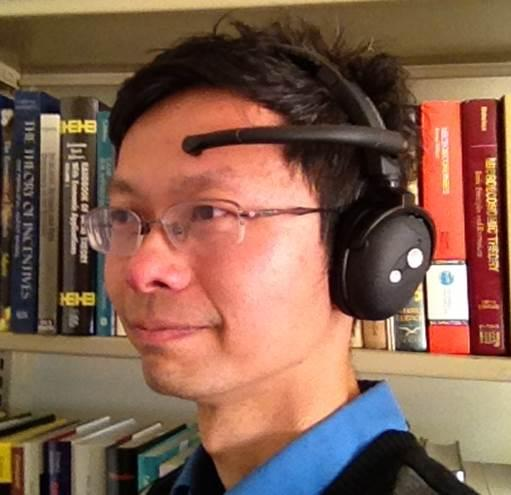
\includegraphics[width=0.5\textwidth]{john_chuang}
    \caption{Professor John Chuang with the Neurosky MindSet brainwave sensor.}
\end{figure}
\chapter{2. Using Brain Waves as New Biometric Feature for Authenticating a Computer User in Real Time}
\href{http://www.cscjournals.org/manuscript/Journals/IJBB/volume7/Issue1/IJBB-211.pdf}
Using brain waves as a biometric Feature for Authenticating was proposed by Kusuma Mohanchandra, Lingaraju G M, Prashanth Kambli \& Vinay in the International Journal of Biometrics and Bioinformat. In this work it has been proved that the brain-wave pattern of every individual is  unique and the signals captured through the  EEG can be used for biometric authentication. This research team used an EEG EPOC headset with 14 channels to measure the brain waves. The collected data, containing the fusion of delta, alpha, theta, beta and gama brain waves, was merged with the aim to create a way to authenticate the user.

There are three basic forms of authentication; something-you-have, something-you-know, and something-you-are.
\begin{itemize}
\item Something-you-have can be objects like a key or passport and people have to be very careful not to loose the object or get it stolen.
\item Something-you-know is based on secret knowledge like passwords or PIN codes and the secret must never be written down, forgotten, or told to others.
\item Something-you-are involves person specific features like fingerprints, voice, face, and gait. Authentication based on such features is called biometric authentication. Brain wave based authentication is a combination of something-you-know and something-you-are when the person involved has to think about something specific, but it can also be just something-you-are when the brain waves are used directly as a biometric.
\end{itemize}
 
The most important part of any authentication system is that true identities (clients) are verified and that false identities (impostors) are rejected. In a password system the password is either right or wrong, but with biometric authentication there is an uncertainty involved because the equipment that  measure the biometric feature rarely provide exactly the same data twice. The reason is that external parameters like finger placement, head rotation, facial hair, location etc are present. The challenge is to overcome these problems in such a way that even two slightly different sets of data can be verified to originate from the same person. There is usually a threshold that decide how different
two different sets of data is allowed to be before they are rejected, and as a consequence there is a chance that some clients are falsely rejected and some impostors are falsely verified.
Biometric authentication therefore introduce two error rates; False Non-Match Rate (FNMR), the rate at which clients are falsely rejected by the system, and False Match Rate (FMR), the rate at which impostors are falsely verified by the system. As such the main problem in this thesis is two compare two or more EEG signals and decide whether they are from the same person or not, and get as low FNMR and FMR as possible.

\chapter{3. Google Glass hack allows brainwave control}
After Google has released his Google Glass, a company called This Place, has developed a app to control the glass over brain waves. But the app alone is not enough to control the glass with the power of your mind. Normally the Goggle Glass is controlled over voice commands or over a touchpad built into the side of the device. To control the device with brain waves This Place combine the Google Glass with the Neurosky MindWave headset. The Neurosky MindWave is an EEG-headset to detect brain waves. This is one of the first devices for consumers. Normally this headset will be used to train your brain and it will be delivered with a hand full games. After combining the two devices, the company begins to testing what kind of brain waves they could detect. For this reason they create a simple app which implements a counter starting at 0. When the user concentrated, the app begin counting upwards towards 50. When the user starts to relaxe, the counter began returning to 0. After this successfully test, they want to develop an app to show a real-world use. So they developed MindRDR. It allows a user to take a photo and share it over Twitter only to use his mind. Very important to know is that the brain waves only activate the camera app at Google Glass and take a photo. The settings for Twitter were set before. They released their software for free, in hope that other developers can adapt it for other uses.

\subsection{Relation to the international scientific work in the field (international status of the research)}
The brain consists of billions of brain cells called neurons. This neurons have to communicate with each other. For this communication the neurons use electricity called brain waves. This communication is producing a lot of brain waves, which can be detected using sensible sensors such as an EEG. The first person, who confirm the existence of brain waves and perform the first tests was Hans Berger. There are five different kinds of brain waves and all of them are directly connected to what a person is thinking, doing and feeling.

\begin{itemize}
 \item Gamma (27 Hz and up)
 \item Beta (12 Hz - 27 Hz)
 \item Alpha (8 Hz - 12 Hz)
 \item Theta (3 Hz - 8 Hz)
 \item Delta (0.2 Hz - 3 Hz)
\end{itemize}

The very beginning of the existence of brain wave based authentication systems dates back to the 1960's when Vogel discovered a connection between a person's EEG signals and his/her genetic code(DNA). It was proved that every person owns unique brainwaves and it possible to identify a person through his brainwaves. Identical twins where shown to have the same EEG patterns in the same situations and even changes related to aging were similar. 


This was also explored by Benedicenti L., Koles’ Z., Mahovsky J., \& Paranjape, R. in the year 2001. This researchers used EEG directly as a biometric and their work showed some promising results on this field.


EEG based person authentication was first proposed by Marcel and Millan in 2007 in “Person authentication using brainwaves (EEG) and maximum a posteriori model adaption”. They proposed the use of  Power Spectral Density as the feature, and a statistical framework based on Gaussian Mixture  Models (GMM) and Maximum A Posteriori Model (MAP) Adaptation on speaker and face  authentication. The potential of their method is shown by simulations using strict train/test protocols and results. 

In 2001 Poulos, Alexandris and Evangelou performed person identification based on spectral information and presented their results in their work: “On the use of EEG features towards oersin identification via neural networks”. To prove the connection between a person's EEG and genetically specific information, this researchers did experiments with the EEG data of healthy individuals. The proposed method has had a success rate of 80 percent to 100 percent showing that the EEG holds genetic information, which can be used for person identification.


Furthermore, a novel two-stage biometric authentication method was proposed by Palaniappan in 2008 (“Two-stage biometric authentication method using thought activity brain waves”). Their results show that the combination of two-stage authentication with EEG features has good potential as a biometric as it is highly resistant to fraud.

\subsection{Description and critical discussion of related scientific work}
The approaches that have been discussed above have succeeded to prove the connection between a person's DNA and her/his brain waves. The approaches clearly show that every single person possesses unique brain waves, which can be used to identify a person. However, a large disadvantage of all of this approaches is that they require the user to wear a big headset with an electrode going across his/her forehead. None of this approaches has succeeded in measuring brain waves from different body parts in order to enable a smaller headset and therefore make it easier for the user to use it in their everyday life.


\note{
\begin{itemize}
\item {\em Length: 2-5 pages}
\item What results and approaches have already been presented in this or related areas?
\item Relation to the international scientific work in the field (international status of the research)
\item Description and critical discussion of related scientific work
\end{itemize}
}

% --------------------------------------------------------------
\section{Method}
\label{sect:method}

\note{
\begin{itemize}
\item {\em Length: 2-5 pages}
\item {\bf How?}
\item How should the expected results be achieved?
\item What method(s) will be applied? (e.g., empirical study, user-centered design, prototype implementation,...)
\item Description of the methods.
\item Justifications for chosen methods.
\end{itemize}
}

% --------------------------------------------------------------
\section{Detailed description of the workpackages}
\label{sect:workplan}

\note{
\begin{itemize}
\item {\em Length: 2-4 pages}
\item Structuring the project into self-contained parts.
\item Additional verbal descriptions.
\item Work packages
    \begin{itemize}
    \item title
    \item goal(s)
    \item description
    \item expected results
    \item responsible person(s)
    \item dependencies
    \end{itemize}
\end{itemize}
}

% --------------------------------------------------------------
\section{Time plan (Gantt chart)}
\label{sect:timeplan}

\note{
\begin{itemize}
\item {\em Length: 1-2 pages}
\item Realistic estimation of schedule based on workpackages.
\item Including milestones (not only when but also what is to be achieved for each milestone).
\item Generation of a Gantt chart. (Including phases, milestones, buffer times, critical areas, etc.)
\end{itemize}
}

% --------------------------------------------------------------
\section{Human resources / team}
\label{sect:team}

\note{
\begin{itemize}
\item {\em Length: 1-2 pages}
\item Description of the team that is needed to carry out the project. (For the execution phase of the project, not the planning phase.)
\item How many people?
\item To what extent are individual members needed?
\item What knowledge, skills, and experiences are needed for each member?
\item Demonstrate that the members will be able to carry out the project successfully.
\item Work structure
	\begin{itemize}
	\item     Who will lead the project?
	\item     How do they work together?
	\item     Management and coordination
		\begin{itemize}
		\item 	        What communication structures will be established? (e.g., mailing list, blog, CMS, CVS, ...)
		\item 	        How often will meetings take place? (Who will participate?)
		\item 	        How will the work be documented?
		\item 	        How will information be stored and shared?
		\end{itemize}
	\end{itemize}
\item Cooperations
	\begin{itemize}
	\item     Will external cooperators be part of the project? (e.g., other research institutions or companies)
	\item     What is their role?
	 \item    Why are they needed?
	\end{itemize}
\end{itemize}
}

% --------------------------------------------------------------
\section{Costs}
\label{sect:costs}

\note{
\begin{itemize}
\item {\em Length: 2-3 pages}
\item Rough estimation of cost in form of calculation (table(s)) + descriptive text.
\item Justification for the personnel and non-personnel costs (equipment, material, travel and other costs)
\item An Excel template is provided as supplementary material to support budgeting.
\item Personnel costs
	\begin{itemize}
	\item     Justification for the personnel to be assigned to the project (type of position(s), description of nature of work, length and extent of involvement in the project)
	\item     The application should include all persons who will be required for the proposed project (project lead, researchers, developers, advisory board, etc.). The available legal categories of employment are contracts of employment for full- or part-time employees (DV) and reimbursement for work on an hourly basis (GB). In addition, a part-time contract of employment (DV 50\%, ``studentische Mitarbeiter'') may be requested for people who have not yet completed a Master or Diploma program (Diplom) in the relevant subject.
	 \item    The justification of the requested personnel should contain:
		\begin{itemize}
		\item 	        description of type of work;
		\item 		        extent of involvement (part-time contracts are permitted).
		\end{itemize}
	\item Exact numbers of employment categories can be found on the FWF Website (\href{http://www.fwf.ac.at/de/projects/personalkostensaetze.html}{http://www.fwf.ac.at/de/projects/personalkostensaetze.html})
	\end{itemize}
\item Equipment costs
	\begin{itemize}
	\item     Indicate reasons for equipment costs. The ``scientific equipment'' category includes instruments, system components, costs for the use of software required by the project and other durable goods provided the cost per item (including VAT) exceeds EUR 1,500.00.
	\end{itemize}
\item Material costs
	\begin{itemize}
	\item     This category encompasses consumables and smaller pieces of equipment where the cost per item is below EUR 1,500.00 including VAT. The calculation of requested material costs should be justified with reference to the schedule, work plan and experimental plan. Experience with previous projects should be taken into account.
	\end{itemize}
\item Travel costs
	\begin{itemize}
	\item     Funding may be requested for the costs of project-specific travel and accommodation, field work, expeditions, etc. Applicants are to provide a detailed travel (cost) plan broken down by project participant. For brief stays, the calculation of the travel and accommodation costs should be based on the federal regulations governing travel costs (RGV). The RGV rates governing Austria and abroad may be found in the FAQs on the FWF Website (\href{http://www.fwf.ac.at/de/faq/reisegebuehrenvorschrift.html}{http://www.fwf.ac.at/de/faq/reisegebuehrenvorschrift.html}). For longer stays an appropriate and comprehensible cost plan should be prepared.
	\end{itemize}
\item Other costs
	\begin{itemize}
	\item     Independent contracts for work and services (costs for work of clearly defined scope and content assigned to individuals, provided that this is scientifically justifiable and economical)
    	\item     Costs that cannot be included under personnel, equipment, material or travel costs, such as:
		\begin{itemize}
		\item         reimbursement of costs towards or for the use of research facilities, e.g. of large-scale research facilities (project-specific 'equipment time'). Applicants should obtain and submit multiple offers;
		\item         costs for project-specific work carried out outside the applicant's research institution (e.g. for analysis work performed elsewhere, for interviews, for sample collection, for preparation of thin slices etc.). Applicants should obtain and submit multiple offers;
		\item         honoraria for test persons;
		\end{itemize}
	\end{itemize}
\end{itemize}
}

% --------------------------------------------------------------
\section{Expected implications and risks}
\label{sect:implication-risk}

\note{
\begin{itemize}
\item {\em Length: 1-2 pages}
\item Importance of the expected results for the discipline
	\begin{itemize}
	\item     To what extent does the proposed research address important challenges?
	\end{itemize}
\item Importance of the expected results for other areas
\item What are possible risks of the project and how can they be alleviated?
	\begin{itemize}
	\item     What factors could lead to a failure of the project?
	\item     Which factors or persons could support the project and increase the chance for success?
	\item     What if important team members leave the project?
	\end{itemize}
\end{itemize}
}

% --------------------------------------------------------------
\section{Ethical considerations \& security issues}
\label{sect:ethics-security}

\note{
\begin{itemize}
\item {\em Length: 1-2 pages}
\item Provide a brief explanation of the ethical issue involved and how it will be dealt with appropriately.
\item Are there any security-sensitive issues that apply to your proposal?
\end{itemize}
}

% --------------------------------------------------------------
% APPENDIX
\begin{appendix}

\pagebreak

% --------------------------------------------------------------
% References
\phantomsection
\addcontentsline{toc}{section}{References}

\bibliographystyle{apalike}
\bibliography{biblography}

\pagebreak

% --------------------------------------------------------------
% Abbreviations
\section*{Abbreviations}
 \addcontentsline{toc}{section}{Abbreviations}
 
 \begin{description}
  \item[MSWP] Management von Software Projekten
  \item[WP] Work Package
 \end{description}

\end{appendix}


\end{document}
